% Drawing 138/04-4 -- folder 138, batch 04, archive page 76 (PDF page 77).
% Transcription: deux diagrammes en éventail. À gauche : $R$ au sommet, quatre flèches $p\colon R \to S$, $q'\colon R \to A$, $q''\colon R \to A$, $r\colon R \to F$. À droite, le même avec $R^{\circ} = R$, $p^{\circ} = p$, $q'^{\circ}$, $q''^{\circ}$ et $q^{\circ} = q \circ \sigma_2$ ; sous $A$, « $q' \circ \sigma_2$ » ; les indications sur les flèches du milieu sont surchargées.
% Kind: fan diagrams (arrows from R). Method 2 (schematic redraw from the facsimile). Status: partial.
% Notes: Two fan-shaped diagrams, the bbox widened so that the right one is whole (it now includes F and the labels at the right). Left: R at the top, four curved arrows p: R -> S, q': R -> A, q'': R -> A (bulging left and right), r: R -> F. Right: « R° = R » at the top, p° = p to S, two arrows to A, the arrow q° = q o sigma_2 to F; « q' o sigma_2 » written under the right end, beside A. Labels of the middle arrows as read: q'° and q'' between the first two (an overinked sign between them, which may be « = », is not set), q''° on the third arrow (the overinked scribble after it is not set). Still differs: the left one of the two middle arrows of the right fan is overinked and partly a reading; the short stroke before « q' o sigma_2 » is left out; the black band at the top is the edge of the sheet. Would be tikz-cd in a transcription; kept as a redraw because the arrows are curved and stacked. Nothing is struck. Redrawn 2026-11-09 (issue 128): to check again.
% Coordinates: 1 unit = 1 mm = 1/100 of the crop width (bbox in page fractions: [0.12, 0.05, 0.56, 0.16]).
% Redrawn by Claude (claude-opus-5-5), issue #73, 2026-11-09; not checked by a human; not compiled (no TeX in the session).
% Rights: reproduces part of the work -- behind RENDER_TRANSCRIPTS, never published by itself.
\documentclass[tikz,border=3pt]{standalone}
\usepackage{amsmath,amssymb}
\usetikzlibrary{patterns,arrows.meta}
\tikzset{pencil/.style={black!45}, struck/.style={black!35}, mark/.style={circle,draw,inner sep=1.3pt}, pt/.style={circle,fill,inner sep=0.9pt}, opt/.style={circle,draw,fill=white,inner sep=1.1pt}}
\begin{document}
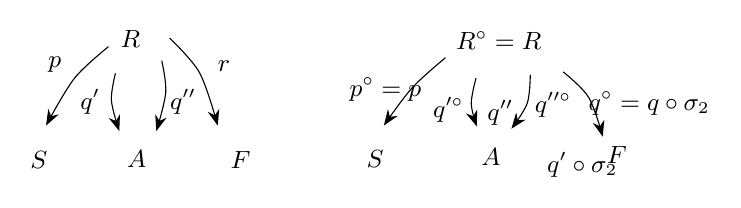
\begin{tikzpicture}[x=1mm,y=1mm,line cap=round,line join=round,font=\scriptsize]
\node[inner sep=1pt] at (24.6,-12.2) {\small $R$};
\node[inner sep=1pt] at (13,-27.6) {\small $S$};
\node[inner sep=1pt] at (25.4,-27.5) {\small $A$};
\node[inner sep=1pt] at (38.6,-27.6) {\small $F$};
\draw[-{Stealth[length=2mm]}] plot[smooth, tension=0.55] coordinates {(21.8,-13.2) (17.5,-17.2) (13.9,-23.2)};
\node[inner sep=1pt] at (15,-15.5) {\small $p$};
\draw[-{Stealth[length=2mm]}] plot[smooth, tension=0.55] coordinates {(22.7,-16.6) (22.2,-20) (23.2,-23.9)};
\node[inner sep=1pt] at (19.5,-20.2) {\small $q'$};
\draw[-{Stealth[length=2mm]}] plot[smooth, tension=0.55] coordinates {(28.6,-15) (29.1,-19) (27.9,-23.9)};
\node[inner sep=1pt] at (31.3,-20.2) {\small $q''$};
\draw[-{Stealth[length=2mm]}] plot[smooth, tension=0.55] coordinates {(29.6,-12.1) (33.4,-16.5) (35.7,-23.2)};
\node[inner sep=1pt] at (36.5,-15.6) {\small $r$};
\node[inner sep=1pt] at (71.4,-12.4) {\small $R^{\circ}=R$};
\node[inner sep=1pt] at (55.7,-27.4) {\small $S$};
\node[inner sep=1pt] at (70.4,-27.2) {\small $A$};
\node[inner sep=1pt] at (86.4,-27) {\small $F$};
\draw[-{Stealth[length=2mm]}] plot[smooth, tension=0.55] coordinates {(64.6,-14.6) (60.4,-18.4) (56.8,-23.2)};
\node[inner sep=1pt] at (57,-18.6) {\small $p^{\circ}=p$};
\draw[-{Stealth[length=2mm]}] plot[smooth, tension=0.55] coordinates {(68.5,-17.2) (67.9,-20.4) (68.6,-23.3)};
\node[inner sep=1pt] at (65,-21.2) {\small $q'^{\circ}$};
\node[inner sep=1pt] at (71.6,-21.6) {\small $q''$};
\draw[-{Stealth[length=2mm]}] plot[smooth, tension=0.55] coordinates {(75.4,-16.8) (75,-20.4) (73,-23.6)};
\node[inner sep=1pt] at (78.3,-20.6) {\small $q''^{\circ}$};
\draw[-{Stealth[length=2mm]}] plot[smooth, tension=0.55] coordinates {(79.6,-16.4) (82.8,-19.6) (84.6,-24.6)};
\node[inner sep=1pt] at (90.5,-20.4) {\small $q^{\circ}=q\circ\sigma_2$};
\node[inner sep=1pt] at (82,-28.2) {\small $q'\circ\sigma_2$};
\end{tikzpicture}
\end{document}
